%% 4 positon, etc.

%% vertices (when start talking about multiple ones) are SORTED, biggest ones first.

Beim Labeling der Knoten sind als geometrische Repräsentation ein Kreis, das heißt, $x,y$-Koordinaten
und ein Radius, sowie der entsprechende Name des Knotens durch die Daten von \texttt{iGraph.js} gegeben.

Nun ist es Aufgabe des Labelings, den Text des Labels erkennbar und visuell ansprechend in Nähe des dazugehörigen Knotens zu platzieren.
Die Breite und die Höhe eines Labels werden von der ausgewählten Schriftart (siehe \hyperref[sec:configuration]{Konfiguration}) beeinflusst.
Aktuell ist die Höhe auf eine Zeile begrenzt in der Implementation.
Die Breite eines Labels hängt zusätzlich von dem entsprechenden Namen bzw. der Anzahl der Buchstaben ab.

So ergeben sich die Höhe und Breite des Labels (sowie der Text selbst) und es muss eine Position in $x,y$-Koordinaten in Abhängigkeit
von dem entsprechenden Knoten gefunden werden.

Die Reihenfolge des Labelings ergibt sich aus einer einmaligen Sortierung.
Diese ist absteigend und sortiert nach der Größe der Radien der Knoten.
Ein größerer Radius steht für eine höhere Relevanz, denn er bedeutet mehr Nachbarn und daher sind diese Knoten vom größerem Interesse.

Zur Generierung der Position eines potentiellen Labels werden nacheinander verschiedene Verfahren verwendet, um möglichst effizient Labelpositionen zu generieren
mit möglichst wenig Überdeckung der einzelnen potentiellen Positionen und so, dass niemals der dazugehörige Knoten überdeckt wird:

\subsubsection{4-Position-Model}
\label{subsubsec:4pos}
Das 4-Position-Model positioniert die potentiellen Labels möglichst nahe an dem korrespondieren Knoten in den Himmelsrichtungen Nord-Ost, Nord-West, Süd-Ost und Süd-West.
Die erste Position ist Nord-Ost, also rechts-oben, und von dort an wird entgegen $x,y$-Koordinaten ein weiteres Label generiert (wenn nötig).

Dieses und das nachfolgende Verfahren sind durch die gängigen Standards der Kartografie inspiriert. Auch dort werden eben beschriebene
Positionen generiert, allerdings in leicht veränderter Reihenfolge.\cite{cartography}

\begin{figure}[H]
    \centering
    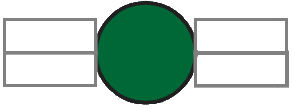
\includegraphics[scale=0.55]{../img/4pos}
    \caption{Labelpositionen im 4-Position-Model von ausgehenden vom dazugehörigen Knoten}
    \label{fig:4pos}
\end{figure}

\subsubsection{8-Position-Model}
\label{subsubsec:8pos}
Im 8-Position-Model werden die potentiellen Labelpositionen in den Haupthimmelsrichtungen Ost, Nord, West, Süd generiert.
Startpunkt ist Osten, also rechts, und wieder wird entgegen des Uhrzeigersinns ggf. ein weiteres Label generiert.

Weiterhin werden die Nord-/Süd-Position im Abstand einer Labelhöhe und die Ost-/West-Position im Abstand einer Labelbreite vom dazugehörigen Knoten positioniert.
Dies wird gemacht, um Überdeckung mit den zuvor im 4-Position-Model generierten Positionen zu vermeiden, da, wenn zuvor das 4-Position-Model schon keine Position finden konnte,
das 8-Position-Model ohne den Abstand dann wahrscheinlich ebenfalls keine Position finden würde.

Das führt dazu, dass vor allem die Ost-/West-Position eher weit entfernt von dem korrespondieren Knoten sind (da Labeltexte bzw. Namen in der Regel eher breit als hoch sind).
Die Kartografie verwendet diese Positionen nicht.\cite{cartography}

In der Implementation wurde dieses Problem dadurch behoben, dass eine "Hilfslinie", als visueller Indikator, das Label mit seinem entsprechenden Knoten verbindet,
sodass die Zugehörigkeit schneller ersichtlich wird.
Diese Technik wird im \hyperref[subsubsec:spiral]{Spiral-Model} nochmals angewandt, da hier dasselbe Problem besteht.

\begin{figure}[H]
    \centering
    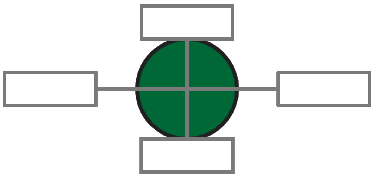
\includegraphics[scale=0.55]{../img/8pos}
    \caption{Labelpositionen im 8-Position-Model von ausgehenden vom dazugehörigen Knoten}
    \label{fig:8pos}
\end{figure}

\subsubsection{Slider-Model}
\label{subsubsec:slider}
Das Slider-Model ist ein aufwendigeres Verfahren als die vorhergehenden beiden. Die Idee hier ist, die Eckpunkte des \hyperref[subsubsec:4pos]{4-Position-Model} zu nehmen
und dann Labelpositionen dazwischen zu generieren, in dem man das potentielle Label stückweise zum nächsten Eckpunkt verschiebt. Der Inkrement-Wert zum Verschieben ist konstant (siehe \hyperref[subsec:consts]{Magic Constants}).

Wie auch beim \hyperref[subsubsec:4pos]{4-Position-Model} in die erste Position die Nord-Ost-Ecke und von dort aus wird parallel zur $y$-Achse die Position verändert bis die Süd-Ost-Ecke erreicht wird.
Da angekommen wird dann parallel zur $x$-Achse in Richtung der Süd-West-Ecke verschoben, usw.

Das Verschieben erfolgt hier offensichtlich im Uhrzeigersinn, um dem Trend der vorherigen beiden Verfahren entgegenzuwirken.

\begin{figure}[H]
    \centering
    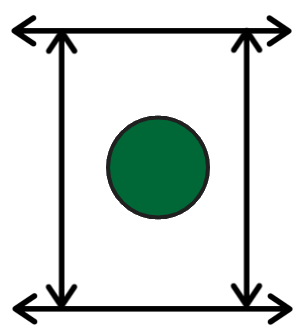
\includegraphics[scale=0.55]{../img/slider}
    \caption{Labelpositionen im Slider-Model von ausgehenden vom dazugehörigen Knoten}
    \label{fig:slider}
\end{figure}

\subsubsection{Spiral-Model}
\label{subsubsec:spiral}

Dieses Verfahren funktioniert gänzlich anders bisher genannten, da diese versuchen, Labelpositionen \textit{kartesisch} zu finden, also durch Verschiebungen
bezüglich der $x,y$-Koordinaten ausgehend vom Mittelpunkt des entsprechenden Knotens. Das Spiral-Model versucht, Labelpositionen \textit{polar} zu finden:
$$ s(m) =
    \left(\begin{array}{c}
              d \cdot \cos (2 \pi \sqrt{\frac{m}{m_{max}}} \cdot c) \\
    \sin (2 \pi \sqrt{\frac{m}{m_{max}}} \cdot c)\end{array}\right) \cdot \sqrt{\frac{m}{m_{max}}} \cdot r,\; \; \; m \in \{1, \dots, m_{max} \}
$$

Das heißt, potentielle Labelposition werden hier spiralförmig generiert, also in ansteigendem Abstand vom dazugehörigen Knoten und in fairer Verteilung hinsichtlich der Richtung der Labels, da die Spirale auch den Winkel fortwährend inkrementiert.
Auch ist die Idee wieder, den Trend von zuvor zu durchbrechen und auf eine unkonventionellere Art Labelposition zu suchen in Regionen, die zuvor noch nicht beachtet wurden.

Die Parameter der Gleichung von Luboschik et al.\cite{main} beeinflussen die Form und Ausrichtung der Spirale:
\begin{itemize}
    \item $d$: Orientierung der Spirale (im/gegen den Uhrzeigersinn), ($d \in \{-1, 1 \}$)
    \item $c$: Krümmung bzw. Anzahl der Rotation der Spirale, ($c \in \mathbb{N}$)
    \item $m_{max}$: Maximalanzahl der Punkte in der Spirale, ($m_{max} \in \mathbb{N}$)
    \item $m$: Der jeweilige $m$-te Punkt der Spirale
\end{itemize}

Ergänzend zu den vorherigen Verfahren ist es sinnvoll, auch das Spiral-Model zu nutzen, da hier schnell Abstand vom dazugehörigen Knoten gewonnen werden kann.
Dies ist wichtig, da die Verfahren zuvor vorrangig in der Nähe des Knotens versuchen, eine Position zu finden. Das Spiral-Model wird aber nur genutzt,
wenn die Verfahren dabei erfolglos geblieben sind.

Wie auch beim \hyperref[subsubsec:8pos]{8-Position-Model} wird, ob des erweiterten Abstands zum korrespondieren Knoten, eine Hilfslinie genutzt,
um die Verbindung für gefundene Labelpositionen und ihre Knoten deutlich zu machen.

\begin{figure}[H]
    \centering
    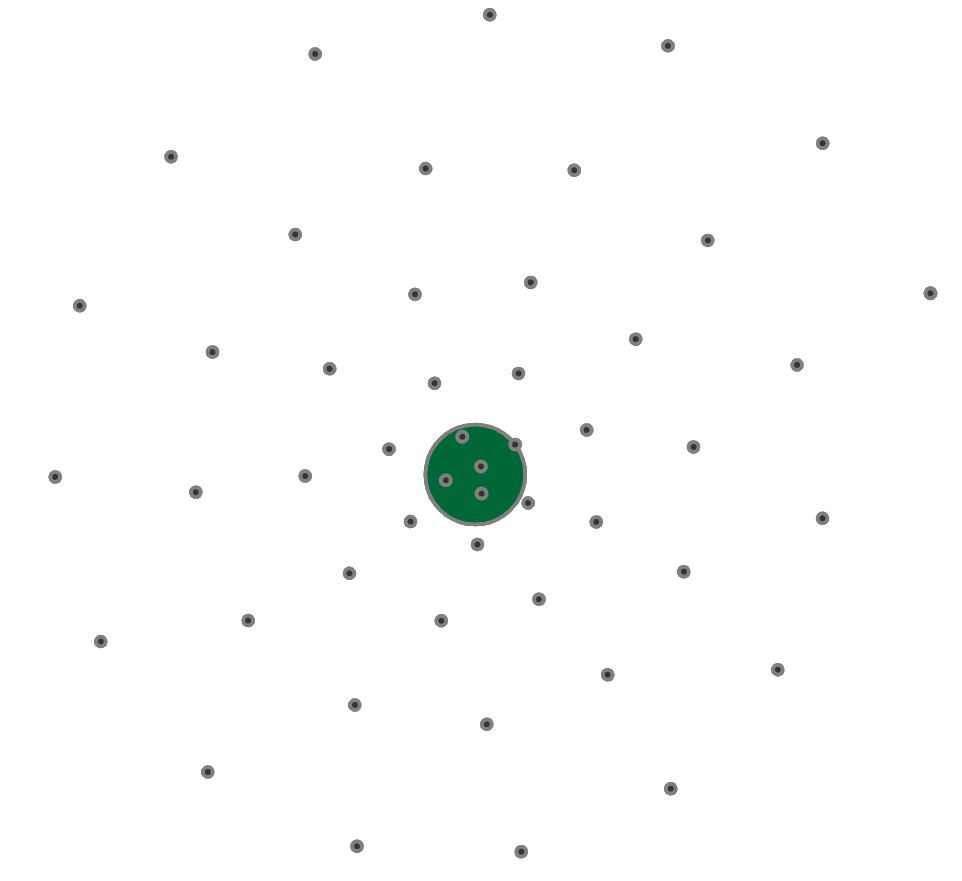
\includegraphics[scale=0.55]{../img/sample}
    \caption{Labelpositionen im Spiral-Model von ausgehenden vom dazugehörigen Knoten.
    Parameter im Beispiel: $m_{max}=50,d=1,c=6,r=500$}
    \label{fig:spiral}
\end{figure}